%
% A header that lets you compile a chapter by itself, or inside a larger document.
% Adapted from http://stackoverflow.com/questions/3655454/conditional-import-in-latex
%
%
%Use \inbpdocument and \outbpdocument in your individual files, in place of \begin{document} and \end{document}. In your main file, put in a \def \ismaindoc {} before including or importing anything.
%
% David Duvenaud
% June 2011
% 
% ======================================
%
%


\ifx\ismaindoc\undefined
	\newcommand{\inbpdocument}{
		\def \ismaindoc {}
		% Use this header if we are compiling by ourselves.
		\documentclass[a4paper,12pt,authoryear,index]{common/PhDThesisPSnPDF}
		\input{common/official-preamble.tex}
		% All my custom preamble stuff.  Shouldn't overlap with anything in official-preamble

\usepackage{nth}
\usepackage{rotating}
\usepackage{array}
%\usepackage{gantt}
\usepackage[hyperpageref]{backref}

		% ************************ Thesis Information & Meta-data **********************

%% The title of the thesis
%\title{Structured Gaussian Process Models} 
%\title{Automatic Model Construction \\ through \\ Structured Gaussian Processes}
%\title{Automatic Model-Building \\ through \\ Structured Gaussian Processes}
%\title{Automatic Modeling \\ with \\ Structured Gaussian Processes}    
\title{Automatic Model Construction \\ with Gaussian Processes}
%\title{Automatic Model Construction}
%\title{Automating Statistical Model Construction}


%\texorpdfstring is used for PDF metadata. Usage:
%\texorpdfstring{LaTeX_Version}{PDF Version (non-latex)} eg.,
%\texorpdfstring{$sigma$}{sigma}

%% The full name of the author
\author{David Kristjanson Duvenaud}

%% Department (eg. Department of Engineering, Maths, Physics)
\dept{Department of Engineering}

%% University and Crest
\university{University of Cambridge}
\crest{\includegraphics[width=0.25\textwidth]{University_Crest}}

%% You can redefine the submission text:
% Default as per the University guidelines: This dissertation is submitted for
% the degree of Doctor of Philosophy
%\renewcommand{\submissiontext}{change the default text here if needed}

%% Full title of the Degree 
\degree{Doctor of Philosophy}
 
%% College affiliation (optional)
\college{Pembroke College}

%% Submission date
\degreedate{June 2014} 

%% Meta information
\subject{LaTeX} \keywords{{LaTeX} {PhD Thesis} {Engineering} {University of
Cambridge}}



		\begin{document}
	}	
	\newcommand{\outbpdocument}[1]{
		%\bibliographystyle{common/CUEDthesis}
		\bibliographystyle{plainnat}
		\bibliography{references.bib}
		\end{document}
	}	
\else
	%If we're inside another document, no need to re-start the document.
	\ifx\inbpdocument\undefined
		\newcommand{\inbpdocument}{}
		\newcommand{\outbpdocument}[1]{}
	\fi
\fi

\inbpdocument

\newcommand{\additivefigsdir}{additive-figures}
\newcommand{\additivetablesdir}{additive-tables}

\chapter{Additive Gaussian Processes}
\label{ch:additive}

In this chapter, we introduce a Gaussian process model of functions which are $\textit additive$.  An additive function is one which decomposes into a sum of low-dimensional functions, each depending on only a subset of the input variables. Additive GPs generalize both Generalized Additive Models, and the standard GP models which use squared-exponential kernels.  Hyperparameter learning in this model can be seen as Bayesian Hierarchical Kernel Learning (HKL).  We introduce an expressive but tractable parameterization of the kernel function, which allows efficient evaluation of all input interaction terms, whose number is exponential in the input dimension.  The additional structure discoverable by this model results in increased interpretability, as well as state-of-the-art predictive power in regression tasks.
%Such functions are sums over functions which each depend only on a subset of the input variables. 

\section{Introduction}
%$f: {\bf x} \mapsto y$

Most regression models in use today restrict the class of allowable functions to be of the form: $g(y) = f(x_1) + f(x_2) + \dots + f(x_D)$.  Popular special cases include logistic regression, linear regression, and Generalized Linear Models (\cite{nelder1972generalized}).  Any function in this family defines a Generalized Additive Model (GAM) (\cite{hastie1990generalized}).   Some extensions of this family, such as smoothing-splines ANOVA (\cite{wahba1990spline}), add terms depending on more than one variable.  However, such models generally become intractable and difficult to fit as the number of terms increases.

At the other end of the spectrum are kernel-based models, which typically allow the response to depend on all input variables simultaneously.  A popular example would be a Gaussian Process model using a squared-exponential (or Gaussian) kernel.  We denote this model as SE-GP.  This model is much more flexible than the GAM, but its flexibility poses a problem:  To the extent that a set of variables is relevant to the output, this model must be highly uncertain about any novel combination of those variables.

In this paper, we introduce a Gaussian process model that generalizes both the GAM and SE-GP.  This is achieved through a kernel which allows additive interactions of all orders, ranging from first order interactions (as in a GAM model) all the way to $D$th-order interactions (as in a SE-GP).  Although this kernel amounts to a sum over an exponential number of terms, we show how to compute this kernel efficiently, and introduce a parameterization which limits the number of hyperparameters to $O(D)$.  A Gaussian process with this kernel function (an additive GP) constitutes a powerful model that allows one to automatically determine which orders of interactions are important.  We show that this model can significantly improve modeling efficacy, and has major advantages for model interpretability.  This model is also extremely simple to implement.

We note that a similar breakthrough has recently been made, called Hierarchical Kernel Learning (HKL) (\cite{DBLP:journals/corr/abs-0909-0844}).  HKL explores a similar class of models, and manages to deal with the possibly exponential number of interaction terms by cleverly selecting only a tractable subset.  However, this method suffers considerably from the fact that cross-validation must be used to set hyperparameters.  In addition, the machinery necessary to train these models is immense.  Finally, on real datasets, HKL is outperformed by the standard SE-GP (\cite{DBLP:journals/corr/abs-0909-0844}).

\section{Gaussian Process Models}

Gaussian processes are a flexible and tractable prior over functions, useful for solving regression and classification tasks (\cite{rasmussen38gaussian}).  The kind of structure which can be captured by a GP model is mainly determined by its \emph{kernel}: the covariance function.  One of the main difficulties in specifying a Gaussian process model is in choosing a kernel which can represent the structure present in the data.  For small to medium-sized datasets, the kernel has a large impact on modeling efficacy.
  

%\subsection{Additivity in a GP}
\begin{figure}
\centering
\begin{tabular}{ccccc|c}
\includegraphics[width=0.2\textwidth]{\additivefigsdir/additive_kernel_sum_p2.pdf} & + & 
\includegraphics[width=0.2\textwidth]{\additivefigsdir/additive_kernel_sum_p1.pdf} &=& 
\includegraphics[width=0.2\textwidth]{\additivefigsdir/additive_kernel.pdf} &
\includegraphics[width=0.2\textwidth]{\additivefigsdir/sqexp_kernel.pdf} \\
$k_1(x_1)$ & & $k_2(x_2)$ & & $k_1(x_1) + k_2(x_2)$ &$k_1(x_1)k_2(x_2)$ \\
1D kernel & & 1D kernel & & 1st order kernel & 2nd order kernel \\ 
%& & & & & \\
%(Second Order) & & & & & Additive Kernel \\
$\downarrow$ & & $\downarrow$ & & $\downarrow$ & $\downarrow$  \\
\includegraphics[width=0.2\textwidth]{\additivefigsdir/additive_kernel_draw_sum_p1.pdf}&+& 
\includegraphics[width=0.2\textwidth]{\additivefigsdir/additive_kernel_draw_sum_p2.pdf}&=&
\includegraphics[width=0.2\textwidth]{\additivefigsdir/additive_kernel_draw_sum.pdf} &
\includegraphics[width=0.2\textwidth]{\additivefigsdir/sqexp_draw.pdf} \\
$f_1(x_1)$ & & $f_2(x_2)$ & & $f_1(x_1) + f_2(x_2)$ & $f(x_1, x_2)$ \\
draw from & & draw from & & draw from 1st & draw from 2nd\\
1D GP prior & & 1D GP prior & & order GP prior & order GP prior\\
%Draw from product kernel GP prior & Draw from additive kernel GP prior\\
\end{tabular}
\caption{A first-order additive kernel, and a product kernel.  Left: a draw from a first-order additive kernel corresponds to a sum of draws from one-dimensional kernels.  Right: functions drawn from a product kernel prior have weaker long-range dependencies, and less long-range structure.
%In this example, both kernels are composed of one dimensional squared-exponential kernels, but this need not be the case in general.
}
\label{fig:kernels}
\end{figure}

Figure \ref{fig:kernels} compares, for two-dimensional functions, a first-order additive kernel with a second-order kernel. We can see that a GP with a first-order additive kernel is an example of a GAM:  Each function drawn from this model is a sum of orthogonal one-dimensional functions.  Compared to functions drawn from the higher-order GP, draws from the first-order GP have more long-range structure.

  %The only weaknesses with this method are due to over-fitting the kernel hyperparameters, the kernel not being rich enough to capture the structure exhibited by the data, or due to the optimization process not finding the global optima of the hyperparameters.

%\subsection{Additivity in the wild}

We can expect many natural functions to depend only on sums of low-order interactions.  For example, the price of a house or car will presumably be well approximated by a sum of prices of individual features, such as a sun-roof.  
%Other features of the object may depend on the size of the object to jointly determine the price.  
Other parts of the price may depend jointly on a small set of features, such as the size and building materials of a house.
Capturing these regularities will mean that a model can confidently extrapolate to unseen combinations of features.


%\subsection{Additive Covariance}

%Figure \ref{fig:draws} shows that functions drawn from sqexp prior in high dimensions can have tons of zero crossings, and thus will take alot of data to learn.

%\subsection{Why additive functions can be expected to be a good model}

\section{Additive Kernels}
%\subsection{Definition}


We now give a precise definition of additive kernels.  We first assign each dimension $i \in \{1 \dots D\}$ a one-dimensional \emph{base kernel} $k_i(x_i, x'_i)$.  We then define the first order, second order and $n$th order additive kernel as:
\begin{eqnarray}
k_{add_1}({\bf x, x'}) & = & \sigma_1^2 \sum_{i=1}^D k_i(x_i, x_i') \\
k_{add_2}({\bf x, x'}) & = & \sigma_2^2 \sum_{i=1}^D \sum_{j = i + 1}^D k_i(x_i, x_i') k_j(x_j, x_j') \\
k_{add_n}({\bf x, x'}) & = & \sigma_n^2 \sum_{1 \leq i_1 < i_2 < ... < i_n \leq D} \prod_{d=1}^N k_{i_d}(x_{i_d}, x_{i_d}')
%k_{add_D}({\bf x, x'}) & = & \sigma_D^2 \prod_{d=1}^D k_{d}(x_{d}, x_{d}')
\end{eqnarray}
where $D$ is the dimension of our input space, and $\sigma_n^2$ is the variance assigned to all $n$th order interactions. The $n$th covariance function is a sum of ${D \choose n}$ terms.  In particular, the $D$th order additive covariance function has ${D \choose D} = 1$ term, a product of each dimension's covariance function:
\begin{equation}
k_{add_D}({\bf x, x'}) = \sigma_D^2 \prod_{d=1}^D k_{d}(x_{d}, x_{d}')
\end{equation}
In the case where each base kernel is a one-dimensional squared-exponential kernel, the $D$th-order term corresponds to the multivariate squared-exponential kernel:
\begin{equation}
%\resizebox{\textwidth}{!}{$
k_{add_D}({\bf x, x'}) = \sigma_D^2 \prod_{d=1}^D k_{d}(x_{d}, x_{d}') = \sigma_D^2 \prod_{d=1}^D \exp \Big( -\frac{ ( x_{d} - x_{d}')^2}{2l^2_d} \Big) = \sigma_D^2  \exp \Big( -\sum_{d=1}^D \frac{ ( x_{d} - x_{d}')^2}{2l^2_d} \Big)
%$}
\end{equation}
also commonly known as the Gaussian kernel.  The full additive kernel is a sum of the additive kernels of all orders.
%
\subsection{Parameterization}

The only design choice necessary in specifying an additive kernel is the selection of a one-dimensional base kernel for each input dimension.  Any parameters (such as length-scales) of the base kernels can be learned as per normal by maximizing the marginal likelihood of the training data.  

In addition to the hyperparameters of each dimension-wise kernel, additive kernels are equipped with a set of $D$ hyperparameters $\sigma_1^2 \dots \sigma_D^2$ controlling how much variance we assign to each order of interaction.  These ``order variance'' hyperparameters have a useful interpretation:  The $d$th order variance hyperparameter controls how much of the target function's variance comes from interactions of the $d$th order.
%
%% --- Automatically generated by hypers_to_latex.m ---
% Exported at 03-Jun-2011 00:23:44
\begin{table}[h]
\caption{{\small
Hyperparameters for concrete dataset.
}}
\label{tbl:concrete}
\begin{center}
\begin{tabular}{r | r r r r r r r r}
Variable: & cement  & slag  & ash  & water  & plast.  & coarse  & fine  & age  \\ \hline
Sq-exp lengthscale & $3.53$  & $3.90$  & $7.13$  & $1.17$  & $3.94$  & $13.61$  & $2.82$  & $0.54$  \\ 
\hline
Additive lengthscale & $1.42$  & $1.57$  & $3.00$  & $0.08$  & $0.52$  & $298.00$  & $1.46$  & $0.11$  \\
\hline
Order of interaction: & \nth{1} & \nth{2} & \nth{3} & \nth{4} & \nth{5} & \nth{6} & \nth{7} & \nth{8} \\
Additive order variance & $70.6$\% & $13.3$\% & $13.8$\% & $2.3$\% & $0.0$\% & $0.0$\% & $0.0$\% & $0.0$\% \\ \hline
\end{tabular}
\end{center}
\end{table}
% End automatically generated LaTeX

%Table \ref{tbl:concrete} gives an example of hyperparameters learnt by both a SE-GP, and by those learnt by an additive GP whose base kernels are one-dimensional squared exponential kernels.  In this case, the 1st, 2nd and 3rd-order interactions contribute most to the final function.
%
%
Table \ref{tbl:all_orders} shows examples of normalized order variance hyperparameters.
\input{\additivetablesdir/all_orders_table.tex}

On different datasets, the dominant order of interaction estimated by the additive model varies widely.An additive GP with all of its variance coming from the 1st order is equivalent to a GAM; an additive GP with all its variance coming from the $D$th order is equivalent to a SE-GP.
%
% We can see that the length-scales learnt are not necessarily the same.  This is because, in a normal ARD-style kernel, the length-scale of a dimension is conflated with the variance of the function along that dimension.  The additive kernel separates these two hyperparameters.
%
%This table lets us examine the relative contribution of each order of interaction to the total function variance.  Again, the ARD kernel is equivalent to an additive kernel in which all the variance is constrained to arise only from the highest-order interactions.

\subsubsection{Model Selection}

Because the hyperparameters can specify which degrees of interaction are important, the additive GP is an extremely general model.  By optimizing these hyperparameters, we are approximately performing weighted model selection over a set of $D$ models.  If the function we are modeling is, in fact, decomposable into a sum of low-dimensional functions, our model can discover this fact (see Figure \ref{fig:synth2d}) and exploit it.  If this is not the case, the hyperparameters can specify a suitably flexible model.
%In the limit of infinite data, a product kernel and its all-subsets expansion will converge to the same mean function (proof?).  However, in the medium-data regime, the additive kernel can discover structure in the functions it is modeling that the product kernel cannot.

%The expected number of zero crossings is $O(k^d)$ for product kernels (sqexp), $O(kd)$ for first-order additive, and $O\left(k  {d \choose r}\right)$ for $r$th order additive functions. [Conjecture]

%To push the analogy, using a product kernel is analogous to performing polynomial regression when we are forced to use a high-degree polynomial, even when the data do not support it.  One could also view the Gaussian kernel as one which makes the pessimistic assumption that the function we are model can vary independently for each new combination of variables observed.
\subsubsection{Interpretability}

As noted by \cite{plate1999accuracy}, one of the chief advantages of additive models such as GAM is their interpretability, since a high-dimensional function is decomposed into a series of one- or two-dimensional functions.  Plate also notes that by allowing high-order interactions as well as low-order interactions, one can trade off interpretability with predictive accuracy.  In the case where the hyperparameters indicate that most of the variance in a function can be explained by low-order interactions, it is useful and easy to plot the corresponding low-order functions, as in Figure \ref{fig:interpretable functions}. 

\begin{figure}[h]
\centering
\begin{tabular}{ccc}
\includegraphics[width=0.3\textwidth]{\additivefigsdir/interpretable_1st_order1.pdf} &
\includegraphics[width=0.3\textwidth]{\additivefigsdir/interpretable_1st_order2.pdf}& 
\includegraphics[width=0.3\textwidth]{\additivefigsdir/interpretable_2nd_order1.pdf}\\
\end{tabular}
\caption{Low-order functions on the concrete dataset.  Left, Centre:  By considering only first-order terms of the additive kernel, we recover a form of Generalized Additive Model, and can plot the corresponding 1-dimensional functions.  Green points indicate the original data, blue points are data after the mean contribution from the other first-order terms has been subtracted.  The black line is the posterior mean of a GP with only one term in its kernel.  Right:  The posterior mean of a GP with only one second-order term in its kernel.}
\label{fig:interpretable functions}
\end{figure}

%\subsection{Allowable Base Kernels}
%Any one-dimensional base kernel is allowable, and each dimension can use a different base kernel.  One could even specify a mixture of base kernels for each dimension, allowing the hyperparameters to specify the mixture weights.

\subsection{Efficient Evaluation of Additive Kernels}
An additive kernel over $D$ inputs with interactions up to order $n$ has $O(2^n)$ terms.  Computing the sum over these terms na\"{i}vely quickly becomes intractable.  In this section, we show how one can evaluate the sum over all terms in $O(D^2)$.

%\subsection{ Elementary Symmetric Polynomials}
The $n$th order additive kernel corresponds to the $n$th \textit{elementary symmetric polynomial} (\cite{macdonald1998symmetric, stanley2001enumerative}), which we denote $e_n$.  For example:  if $\bf x$ has 4 input dimensions ($D = 4$), and if we let $z_i = k_i(x_i,x_i')$, then
\begin{align*}
%k_{a_1}({\bf x, x'}) & = e_0( z_1, z_2, z_3, z_4 ) & = & 1 \\
k_{add_1}({\bf x, x'}) & = e_1( z_1, z_2, z_3, z_4 ) = z_1 + z_2 + z_3 + z_4 \\
k_{add_2}({\bf x, x'}) & = e_2( z_1, z_2, z_3, z_4 ) = z_1 z_2 + z_1 z_3 + z_1z_4 + z_2 z_3 + z_2 z_4 + z_3 z_4 \\
k_{add_3}({\bf x, x'}) & = e_3( z_1, z_2, z_3, z_4 ) = z_1 z_2 z_3 + z_1 z_2 z_4 + z_1 z_3 z_4 + z_2 z_3 z_4 \\
k_{add_4}({\bf x, x'}) & = e_4( z_1, z_2, z_3, z_4 ) = z_1 z_2 z_3 z_4
\end{align*}
The Newton-Girard formulae give an efficient recursive form for computing these polynomials:
\begin{equation}
k_{add_n}({\bf x, x'}) = e_n(z_1,\dots,z_n) = \frac{1}{n} \sum_{k=1}^n (-1)^{(k-1)} e_{n-k}(z_1,\dots,z_D)s_k(z_1,\dots,z_D)
\end{equation}
where $s_k$ is the $k$th {\bf power sum}:
%\begin{equation}
%$s_k(z_1,z_2,\dots,z_n) = z_1^k + z_2^k + \dots + z_D^k = \sum_{i=1}^Dz_i^k$.
$s_k(z_1,z_2,\dots,z_n) = \sum_{i=1}^Dz_i^k$.
%\end{equation}
The Newton-Girard formulae have time complexity $O( D^2 )$, while computing a sum over an exponential number of terms.
%\subsection{Evaluation of Derivatives}

Conveniently, we can use the same trick to efficiently compute all of the necessary derivatives of the additive kernel with respect to the base kernels.  We merely need to remove the kernel of interest from each term of the polynomials:
\begin{align}
\frac{\partial k_{add_n}}{\partial z_j} & = e_{n-1}(z_1,\dots,z_{j-1},z_{j+1}, \dots z_D)
% & = \frac{1}{n-1} \sum_{k=1}^{n-1} (-1)^{(k-1)} e_{n-k-1}(z_1,\dots,z_{j-1},z_{j+1}, \dots z_D)s_k(z_1,\dots,z_{j-1},z_{j+1}, \dots z_D)
\end{align}
This trick allows us to optimize the base kernel hyperparameters with respect to the marginal likelihood.

%  The final derivative is a sum of multilinear terms, so if only one term depends on the hyperparameter under consideration, we can factorise it out and compute the sum with one degree less.
\subsubsection{Computation}
The computational cost of evaluating the Gram matrix of a product kernel (such as the SE kernel) is $O(N^2D)$, while the cost of evaluating the Gram matrix of the additive kernel is $O(N^2D + N^2R^2)$, where R is the maximum degree of interaction allowed (up to D).  In higher dimensions, this can be a significant cost, even relative to the fixed $O(N^3)$ cost of inverting the Gram matrix.
%
However, as our experiments show, typically only the first few orders of interaction are important for modeling a given function; hence if one is computationally limited, one can simply limit the maximum degree of interaction without losing much accuracy.

%\subsection{Code}
Additive Gaussian processes are particularly appealing in practice because their use requires only the specification of the base kernel.  All other aspects of GP inference remain the same.  All of the experiments in this paper were performed using the standard GPML toolbox \footnote{Available at \texttt{http://www.gaussianprocess.org/gpml/code/}}.  Code to perform all experiments is available at the author's website.


\section{Related Work}

\cite{plate1999accuracy} constructs a form of additive GP, but using only the first-order and $D$th order terms.  This model is motivated by the desire to trade off the interpretability of first-order models, with the flexibility of full-order models.  Our experiments show that often, the intermediate degrees of interaction contribute most of the variance.

A related functional ANOVA GP model by \cite{kaufman2010bayesian} decomposes the \emph{mean} function into a weighted sum of GPs. However, the effect of a particular degree of interaction cannot be quantified by that approach. Also, computationally, the Gibbs sampling approach is disadvantageous.
%[Todo:  read and mention  and \cite{friedman1981projection} from Hannes]

%\subsection{Multiple Kernel Learning}

%Our current framework relates to Multiple Kernel Learning in that we are learning the weights in a certain mixture of kernels.  
\cite{christoudias2009bayesian} previously showed how mixtures of kernels can be learnt by gradient descent in the Gaussian process framework.  They call this \emph{Bayesian localized multiple kernel learning}.
However, their approach learns a mixture over a small, fixed set of kernels, while our method learns a mixture over all possible products of those kernels.

\subsection{Hierarchical Kernel Learning}

\begin{figure}
\centering
\begin{tabular}{c|c|c|c}
\hspace{-0.06in} \includegraphics[width=0.23\textwidth]{\additivefigsdir/compare_models/hkl.pdf} \hspace{-0.07in} &
\hspace{-0.06in} \includegraphics[width=0.23\textwidth]{\additivefigsdir/compare_models/gam.pdf} \hspace{-0.07in} &
\hspace{-0.06in} \includegraphics[width=0.23\textwidth]{\additivefigsdir/compare_models/ard.pdf} \hspace{-0.07in} &
\hspace{-0.06in} \includegraphics[height=0.19\textwidth]{\additivefigsdir/compare_models/additive.pdf} \\
HKL & GP-GAM & Squared-exp GP & Additive GP
\end{tabular}
\caption{
%A comparison of model flexibility between HKL, additive GPs, the GP-Generalized Additive Model, and the squared-exponential GP model.  
Nodes represent different interaction terms, ranging from first-order to fourth-order interactions.  Far left:  HKL can select a hull of interaction terms, but must use a pre-determined weighting over those terms.  Far right: the additive GP model can weight each order of interaction seperately.  Neither the HKL nor the additive model dominate one another in terms of flexibility, however the GP-GAM and the SE-GP are special cases of additive GPs. }
\label{hulls-figure}
\end{figure}

\cite{DBLP:journals/corr/abs-0909-0844} uses a regularized optimization framework to learn a weighted sum over an exponential number of kernels which can be computed in polynomial time.  The subsets of kernels considered by this method are restricted to be a \textit{hull} of kernels.\footnote{In the setting we are considering in this paper, a hull can be defined as a subset of all terms such that if term $\prod_{j \in J} k_j(\bf x, x')$ is included in the subset, then so are all terms $\prod_{j \in J / i} k_j(\bf x, x')$, for all $i \in J$.  For details, see \cite{DBLP:journals/corr/abs-0909-0844}.}
Given each dimension's kernel, and a pre-defined weighting over all terms, HKL performs model selection by searching over hulls of interaction terms.
% \subsubsection{All-subsets kernel with uniform weightings}
In \cite{DBLP:journals/corr/abs-0909-0844}, Bach also fixes the relative weighting between orders of interaction with a single term $\alpha$, computing the sum over all orders by:
\begin{equation}
\label{eqn:uniform}
k_{a}({\bf x, x'}) = v_D^2 \prod_{d=1}^D \left(1 + \alpha k_{d}(x_{d}, x_{d}') \right)
\end{equation}
which has computational complexity $O(D)$.  However, this formulation forces the weight of all $n$th order terms to be weighted by $\alpha^n$.

Figure \ref{hulls-figure} contrasts the HKL hull-selection method with the Additive GP hyperparameter-learning method. Neither method dominates the other in flexibility.  The main difficulty with the approach of \cite{DBLP:journals/corr/abs-0909-0844} is that hyperparameters are hard to set other than by cross-validation.  In contrast, our method optimizes the hyperparameters of each dimension's base kernel, as well as the relative weighting of each order of interaction. 


\subsection{ANOVA Procedures}

\cite{vapnik1998statistical} introduces the support vector ANOVA decomposition, which has the same form as our additive kernel.  However, they recommend approximating the sum over all $D$ orders with only one term ``of appropriate order'', presumably because of the difficulty of setting the hyperparameters of a SVM. \cite{stitson1999support} performed experiments which favourably compared the support vector ANOVA decomposition to polynomial and spline kernels.  They too allowed only one order to be active, and set hyperparameters by cross-validation.
%
%  The order of the kernel, kernel hyperparameters, the allowable regression error $\epsilon$, and the cost hyperparameter $c$ were all set by a lengthy cross-validation process.

%\subsection{Smoothing Splines ANOVA}
A closely related procedure from the statistics literature is smoothing-splines ANOVA (SS-ANOVA) (\cite{wahba1990spline}). An SS-ANOVA model is estimated as a weighted sum of splines along each dimension, plus a sum of splines over all pairs of dimensions, all triplets, etc, with each individual interaction term having a separate weighting parameter.  Because the number of terms to consider grows exponentially in the order, in practice, only terms of first and second order are usually considered.  Learning in SS-ANOVA is usually done via penalized-maximum likelihood with a fixed sparsity hyperparameter.
% estimated by generalized cross-validation\cite{craven1978smoothing}. 
%MARS\cite{friedman1991multivariate} is another spline-based regression method.

In contrast to these procedures, our method can easily include all $D$ orders of interaction, each weighted by a separate hyperparameter. As well, we can learn kernel hyperparameters individually per input dimension, allowing automatic relevance determination to operate.

\subsection{Non-local Interactions}

%In this section we give one motivation for why low-order interactions might help our predictive accuracy.
%
%The SE-GP model relies on local smoothing to make predictions at novel locations.  Recent work by Bengio et. al. discusses the limitations
By far the most popular kernels for regression and classification tasks on continuous data are the squared exponential (Gaussian) kernel, and the Mat\'{e}rn kernels.  These kernels depend only on the scaled Euclidean distance between two points, both having the form: $ k({\bf x, x'}) = f(\sum_{d=1}^D \left( x_{d} - x_{d}' \right)^2 / l_d^2)$.
%\begin{eqnarray}
%k_{se}({\bf x, x'}) & = & v_D^2  \exp \left( -\frac{r^2}{2} \right) \\
%k_{\nu}({\bf x, x'}) & = & \frac{2^{1-\nu}}{\Gamma(\nu)}\left(\sqrt{2\nu}r\right) K_\nu \left(\sqrt{2\nu}r\right)
%\end{eqnarray}
%Where
%\begin{equation}
%$r = \sqrt{\sum_{d=1}^D \left( x_{d} - x_{d}' \right)^2 / l_d^2 }$.
%\end{equation}
\cite{bengio2006curse} argue that models based on squared-exponential kernels are particularily susceptible to the \textit{curse of dimensionality}.  They emphasize that the locality of the kernels means that these models cannot capture non-local structure.  They argue that many functions that we care about have such structure.  Methods based solely on local kernels will require training examples at all combinations of relevant inputs.

\begin{figure}[h]
\centering
\begin{tabular}{cc}
\hspace{-0.25in} \includegraphics[width=0.3\textwidth]{\additivefigsdir/3d_add_kernel_1.pdf} &
\hspace{-0.25in} \includegraphics[width=0.3\textwidth]{\additivefigsdir/3d_add_kernel_2.pdf} \\
1st order interactions & 2nd order interactions \\
$k_1 + k_2 + k_3$ & $k_1k_2 + k_2k_3 + k_1k_3$ \\
\hspace{-0.25in} \includegraphics[width=0.3\textwidth]{\additivefigsdir/3d_add_kernel_3.pdf} & 
\hspace{-0.25in} \includegraphics[width=0.3\textwidth]{\additivefigsdir/3d_add_kernel_321.pdf}\\
3rd order interactions & All interactions \\
 $k_1k_2k_3$ & \\
 (Squared-exp kernel) & (Additive kernel)\\
\end{tabular}
\caption{Isocontours of additive kernels in 3 dimensions.  The third-order kernel only considers nearby points relevant, while the lower-order kernels allow the output to depend on distant points, as long as they share one or more input value.}
\label{fig:kernels3d}
\end{figure}

Additive kernels have a much more complex structure, and allow extrapolation based on distant parts of the input space, without spreading the mass of the kernel over the whole space.  For example, additive kernels of the first order allow strong non-local interactions along every axis.
Figure \ref{fig:kernels3d} compares a squared-exponential kernel with an additive kernel in 3 dimensions.


\section{Experiments}

\subsection{Synthetic Data}

Because additive kernels can discover non-local structure in data, they are exceptionally well-suited to problems where local interpolation fails.  
%[Would this make them good for nonstationary noise?]
\begin{figure}[h]
\centering
\begin{tabular}{cccc}
\hspace{-0.1in}\includegraphics[width=0.24\textwidth]{\additivefigsdir/1st_order_censored_truth.pdf} &
\hspace{-0.1in}\includegraphics[width=0.24\textwidth]{\additivefigsdir/1st_order_censored_ard.pdf}&
\hspace{-0.1in}\includegraphics[width=0.24\textwidth]{\additivefigsdir/1st_order_censored_add.pdf}& 
\hspace{-0.1in}\includegraphics[width=0.24\textwidth]{\additivefigsdir/1st_order_censored_d1d2.pdf}\\ 
True Function & Squared-exp GP & Additive GP & Additive GP \\
 \& data locations & posterior mean & posterior mean & 1st-order functions\\
%\includegraphics[width=0.3\textwidth]{\additivefigsdir/1st_order_censored_data.pdf} &
%\includegraphics[width=0.3\textwidth]{\additivefigsdir/1st_order_censored_d1.pdf}&
%\includegraphics[width=0.3\textwidth]{\additivefigsdir/1st_order_censored_d2.pdf}\\
%Training Data Locations & Estimated 1D $f(x_1)$ & Estimated 1D $f(x_2)$ \\
\end{tabular}
\caption{Long-range inference in functions with additive structure.%  The additive GP is able to discover the additive pattern, and use it to fill in a distant mode.  The ARD kernel can only interpolate, and thus predicts the mean in locations missing data.
}
\label{fig:synth2d}
\end{figure}
%Figure \ref{fig:synth2d} shows a simple experiment demonstrating the ability of additive kernels to discover low-order structure, and to exploit that structure to make predictions about unseen combinations of inputs.
We constructed a dataset to demonstrate this ability in additive GPs, consisting of data drawn from a sum of two axis-aligned sine functions.  The training set is restricted to a small, L-shaped area; the test set contains a peak far from the training set locations.  The additive GP recovered both of the original sine functions (shown in green), and inferred correctly that most of the variance in the function comes from first-order interactions.  Figure \ref{fig:synth2d} shows the results.  The ability of additive GPs to discover long-range structure suggests that this model may be well-suited to deal with covariate-shift problems.

\subsection{Experimental Setup}
%\subsubsection{Learning}

%\subsubsection{Overfitting}
%A multivariate squared exponential kernel has $D + 1$ hyperparameters, while an additive function with one hyperparameter per dimension (e.g., a scale parameter) on each dimension's covariance function will have $D \times 2$ hyperparameters.  Because each additional hyperparameter increases the tendency to overfit, we recommend allowing only one hyperparameter per input dimension. 

%
%Since there always exists a parameterization of the additive function corresponding to the product kernel, we initialize the hyperparameter search for the additive kernel by first learning hyperparameters for the equivalent product kernel.  This ensures that we start our search in a reasonable area of hyperparameter space.
%
%  Results were averaged over 10 cross-validation folds.  To limit the possibility of overfitting, we parametrized each of our one-dimensional kernel functions with only the lengthscale.  
%Note that this parameterization is still more flexible than previous methods (HKL, SS-ANOVA).  % This needs to be double-checked.

%\subsubsection{Initialization}
%We tried 2 different hyperparameterizations, and 3 initialization strategies: \texttt{vo} indicates learning only the variance parameter of each one-dimensional kernel, and \texttt{lo} indicates learning only the lengthscale.  \texttt{grow} indicates that the model was initialized with only 1st-order interactions, and higher interactions were added in stages.  \texttt{ard init} indicates that lengthscales were initialized by first optimizing the hyperparameters of a squared-exp kernel, then copying the lengthscales for use in an additive kernel.
%\subsection{Models}

On a diverse collection of datasets, we compared five different models.  In the results tables below, GP Additive refers to a GP using the additive kernel with squared-exp base kernels.  For speed, we limited the maximum order of interaction in the additive kernels to 10.  GP-GAM denotes an additive GP model with only first-order interactions.  GP Squared-Exp is a GP model with a squared-exponential ARD kernel.  HKL\footnote{Code for HKL available at \texttt{http://www.di.ens.fr/\textasciitilde fbach/hkl/}} was run using the all-subsets kernel, which corresponds to the same set of kernels as considered by the additive GP with a squared-exp base kernel.     

%For all 3 GP models, we allowed 5 multiple restarts for all of our hyperparameter maximization steps, choosing the set of hyperparameters with the highest training-set marginal likelihood.  We ran each hyperparameter search for 500 function evaluations by the usual method of maximizing marginal likelihood, using L-BFGS \cite{nocedal1980updating}.  In addition to kernel hyperparameters, we fit a constant mean function to the data.
For all GP models, we fit hyperparameters by the standard method of maximizing training-set marginal likelihood, using L-BFGS (\cite{nocedal1980updating}) for 500 iterations, allowing five random restarts.  In addition to learning kernel hyperparameters, we fit a constant mean function to the data.
%
In the classification experiments, GP inference was done using expectation propagation (\cite{minka2001expectation}).
 
\subsection{Results}

Tables \ref{tbl:Regression Mean Squared Error}, \ref{tbl:Regression Negative Log Likelihood}, \ref{tbl:Classification Percent Error} and \ref{tbl:Classification Negative Log Likelihood} show mean performance across 10 train-test splits.  Because HKL does not specify a noise model, it could not be included in the likelihood comparisons.

% --- Automatically generated by resultsToLatex2.m ---
% Exported at 19-Jan-2012 10:55:19
\begin{table}[h!]
\caption{{\small
Regression Mean Squared Error
}}
\label{tbl:Regression Mean Squared Error}
\begin{center}
\begin{tabular}{l | r r r r r}
Method & \rotatebox{0}{ bach  }  & \rotatebox{0}{ concrete  }  & \rotatebox{0}{ pumadyn-8nh }  & \rotatebox{0}{ servo }  & \rotatebox{0}{ housing }  \\ \hline
Linear Regression & $1.031$ & $0.404$ & $0.641$ & $0.523$ & $0.289$ \\
GP GAM & $1.259$ & $0.149$ & $0.598$ & $0.281$ & $0.161$ \\
HKL & $\mathbf{0.199}$ & $0.147$ & $0.346$ & $0.199$ & $0.151$ \\
GP Squared-exp & $\mathbf{0.045}$ & $0.157$ & $\mathbf{0.317}$ & $\mathbf{0.126}$ & $\mathbf{0.092}$ \\
GP Additive & $\mathbf{0.045}$ & $\mathbf{0.089}$ & $\mathbf{0.316}$ & $\mathbf{0.110}$ & $\mathbf{0.102}$ \\
\end{tabular}
\end{center}
\end{table}
% End automatically generated LaTeX

\input{\additivetablesdir/reg_table_ll2.tex}
% --- Automatically generated by resultsToLatex2.m ---
% Exported at 03-Jun-2011 00:23:25
\begin{table}[h!]
\caption{{\small
Classification Percent Error
}}
\label{tbl:Classification Percent Error}
\begin{center}
\begin{tabular}{l | r r r r r r}
Method & \rotatebox{0}{ breast }  & \rotatebox{0}{ pima }  & \rotatebox{0}{ sonar }  & \rotatebox{0}{ ionosphere }  & \rotatebox{0}{ liver }  & \rotatebox{0}{ heart }  \\ \hline
Logistic Regression & $7.611$ & $24.392$ & $26.786$ & $16.810$ & $45.060$ & $\mathbf{16.082}$ \\
GP GAM & $\mathbf{5.189}$ & $\mathbf{22.419}$ & $\mathbf{15.786}$ & $\mathbf{8.524}$ & $\mathbf{29.842}$ & $\mathbf{16.839}$ \\
HKL & $\mathbf{5.377}$ & $24.261$ & $\mathbf{21.000}$ & $9.119$ & $\mathbf{27.270}$ & $\mathbf{18.975}$ \\
GP Squared-exp & $\mathbf{4.734}$ & $\mathbf{23.722}$ & $\mathbf{16.357}$ & $\mathbf{6.833}$ & $\mathbf{31.237}$ & $\mathbf{20.642}$ \\
GP Additive & $\mathbf{5.566}$ & $\mathbf{23.076}$ & $\mathbf{15.714}$ & $\mathbf{7.976}$ & $\mathbf{30.060}$ & $\mathbf{18.496}$ \\
\end{tabular}
\end{center}
\end{table}
% End automatically generated LaTeX

\input{\additivetablesdir/class_table_ll2.tex}

The model with best performance on each dataset is in bold, along with all other models that were not significantly different under a paired t-test. The additive model never performs significantly worse than any other model, and sometimes performs significantly better than all other models.  The difference between all methods is larger in the case of regression experiments. The performance of HKL is consistent with the results in \cite{DBLP:journals/corr/abs-0909-0844}, performing competitively but slightly worse than SE-GP.%  This is especially clear in the case of the regression tasks.

Because the additive GP is a superset of both the GP-GAM model and the SE-GP model, instances where the additive GP model performs significantly worse are presumably due to over-fitting, or due to the hyperparameter optimization becoming stuck in a local maximum. % Absence of over-fitting may explain the relatively strong performance of GP-GAM on classification tasks.  
Additive GP performance can be expected to benefit significantly from integrating out the kernel hyperparameters.

\section{Future Work}

The kernel used by \cite{DBLP:journals/corr/abs-0909-0844} is less flexible than ours, but has time complexity $O(N^2 D)$ as opposed to the additive kernel as defined in this chapter.  An experimental evaluation of Gaussian process regression with this kernel would reveal if the all-subsets kernel is a faster alternative to the fully-parametrized GP model.

One difficulty with the current formulation of additive GPs is that the length-scale parameters of the base kernels are use as distance metrics in spaces of different dimension.  Upon examination of the lengthscales of sq-exp GPs and additive GPs, it was found that in the cases where the lower orders contributed the most variance, the length-scale parameters were consistently much smaller than in the cases where the high-order terms dominated.  This is strong evidence that different length-scales are appropriate for different orders of interaction.

An naive solution to this problem would be to multiply the lengthscales of the interaction terms in the $d$th order of interaction by a $\sqrt(d)$.

One tantalizing takeaway from the experimental results presented here is that, for Gaussian process classification (GPC), an additive model using only the first-order interactions is as good or better that full-interaction additive GPs as well as sq-exp GPs.  This result is encouraging because recently, (Yunus et al) demonstrated that inference in first-order additive GPs is possible in $O(ND)$.  In the case of GPC, enforcing only first-order interactions may give a massive gain in speed for essentially no cost in accuracy when using maximum-likelihood estimates for the hyperparameters.

\section{Conclusion}

%We present a simple model which generalizes two widely-used classes of models.  A large increase in modeling power is gained at only modest computational cost.
We present additive Gaussian processes: a simple family of models which generalizes two widely-used classes of models.  Additive GPs also introduce a new type of structure into the GP framework.   Our experiments indicate that such additive structure is present in real datasets, allowing our model to perform better than standard GP models.  In the case where no such structure exists, our model can recover arbitrarily flexible models, as well.

In addition to improving modeling efficacy, the additive GP also improves model interpretability:  the order variance hyperparameters indicate which sorts of structure are present in our model.

Compared to HKL, which is the only other tractable procedure able to capture the same types of structure, our method benefits from being able to learn individual kernel hyperparameters, as well as the weightings of different orders of interaction.  Our experiments show that additive GPs are a state-of-the-art regression model.



\outbpdocument{
\bibliographystyle{plainnat}
\bibliography{references.bib}
qwerty
}

